\chapter{Theory}
\section{Algorithms}
This chapter will take a look at commonly used algorithms in image processing for edge detection, identifying areas of interest and applying them onto pupil detection. At first the algorithms will be discussed and analyzed on possible use cases, individual strengths and weaknesses. To show the nature of the algorithm, the same preprocessed images from the LPW data set are used and therefore it is possible to showcase the results and compare them. The general approach for pupil detection, even tough different algorithms are use, can be summarized by finding the region of interest (ROI), then find pupil edges and finally extract the pupil as ellipse. Depending on the algorithm, the steps can sometimes be extended or even combined. This chapter will therefore also discuss the possible combinations of algorithms. 

\subsection{Fundamental notation}\label{subsec:funda}
Thru out this thesis the following notation is used to descripe the algorithms.
The image with intensity level $I$ is a function 

$f(x,y): \mathbb{\mathbb{N_0} }^2 \rightarrow \mathbb{\mathbb{N_0}}$, where $f(x,y)$ is the intensity $I \in $ [$0,255$] at position $(x,y)$

In image processing there the coordinate system is defined different than in mathematics. The origin is in the upper left corner and the x-axis is pointing to down vertically. The y axis is pointing to the right horizontally. this is shown in figure \ref{fig:coordsystem}.

\begin{figure}[h]
    \centering

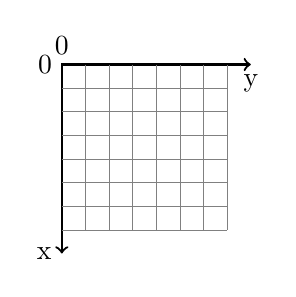
\begin{tikzpicture}[x=0.3cm,y=-0.3cm]
    
    % Draw the x-axis
    \draw[->,thick] (0,8) -- (0,0) -- (8,0) node[below] {y};
    % Draw the y-axis
    \draw[->,thick] (0,0) -- (0,8) node[left] {x};
    % Label the origin
    \node at (0,0) [left] {0};
    \node at (0,0) [above] {0};
    \foreach \x in {1,2,...,7}
    \draw[gray, very thin] (\x,0) -- (\x,7);
  \foreach \y in {1,2,...,7}
    \draw[gray, very thin] (0,\y) -- (7,\y);
  \end{tikzpicture}

    \caption{Coordinate system used in image processing.}
    \label{fig:coordsystem}
\end{figure}

Also important to note it that the image is a discrete function, therefore each intensity value $I$ comes with an quantization error. This is also the case when using an algorithm on the intensity values of the image. So it is not possible to have an exact result, it is always an approximation of the real result.

\subsubsection{Relationship between pixels}
One also important theory in this thesis will be based on relationship between pixels. In this subsection the terms \textbf{neighborhood}, \textbf{adjacency}, \textbf{connectivity}, \textbf{region} and \textbf{boundaries} will be introduced and visualized, so that they can be used in the following chapters. 

\paragraph{Neighborhood}
A pixel $P$ at location $(x,y)$ has two vertical neighbor pixels and two horizontal neighbor pixels in a 2D image. These neighbors are defined as $N_4(P)$ with coordinates: 
\begin{equation}
        N_4(P) = \{(x,y+1),(x,y-1),(x+1,y),(x-1,y)\}
\end{equation}
A pixel $P$ at location $(x,y)$ has four diagonal neighbor pixels in a 2D image. These neighbors are defined as $N_D(P)$ with coordinates:
\begin{equation}
    N_D(P) = \{(x+1,y+1),(x+1,y-1),(x-1,y+1),(x-1,y-1)\}
\end{equation}

Adding the neighbors from $N_4(P)$ and $N_D(P)$ results in the 8-neighborhood $N_8(P)$ of pixel $P$ with coordinates:
\begin{equation}
    N_8(P) = N_4(P) \cup N_D(P)
\end{equation}


    \begin{figure}[ht]
        \centering
        \begin{subfigure}[b]{0.23\textwidth}
            \centering
            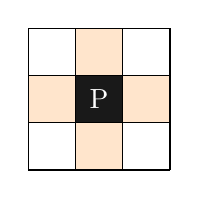
\begin{tikzpicture}[scale=0.6]
                \draw (0,0) grid (3,3);
                \filldraw[fill=orange!20] (1,0) rectangle (2,1);
                \filldraw[fill=orange!20] (1,2) rectangle (2,3);
                \filldraw[fill=orange!20] (0,1) rectangle (1,2);
                \filldraw[fill=orange!20] (2,1) rectangle (3,2);
                \filldraw[fill=black!90] (1,1) rectangle (2,2);
                \node[white] at (1.5,1.5) {P};
            \end{tikzpicture}
            \caption{$N_4(P)$}
            \label{fig:n_4}
        \end{subfigure}%
        \begin{subfigure}[b]{0.23\textwidth}
            \centering
            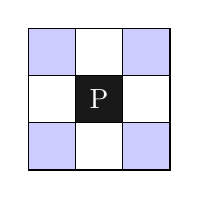
\begin{tikzpicture}[scale=0.6]
                \draw (0,0) grid (3,3);
                \filldraw[fill=blue!20] (0,3) rectangle (1,2);
                \filldraw[fill=blue!20] (2,0) rectangle (3,1);
                \filldraw[fill=blue!20] (0,0) rectangle (1,1);
                \filldraw[fill=blue!20] (2,2) rectangle (3,3);
                \filldraw[fill=black!90] (1,1) rectangle (2,2);
                \node[white] at (1.5,1.5) {P};
            \end{tikzpicture}
            \caption{$N_D(P)$}
            \label{fig:n_d}
        \end{subfigure}%
        \begin{subfigure}[b]{0.23\textwidth}
            \centering
            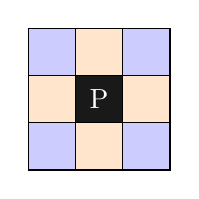
\begin{tikzpicture}[scale=0.6]
                \draw (0,0) grid (3,3);
                \filldraw[fill=blue!20] (0,3) rectangle (1,2);
                \filldraw[fill=blue!20] (2,0) rectangle (3,1);
                \filldraw[fill=blue!20] (0,0) rectangle (1,1);
                \filldraw[fill=blue!20] (2,2) rectangle (3,3);
                \filldraw[fill=orange!20] (1,0) rectangle (2,1);
                \filldraw[fill=orange!20] (1,2) rectangle (2,3);
                \filldraw[fill=orange!20] (0,1) rectangle (1,2);
                \filldraw[fill=orange!20] (2,1) rectangle (3,2);
                \filldraw[fill=black!90] (1,1) rectangle (2,2);

                \node[white] at (1.5,1.5) {P};
            \end{tikzpicture}
            \caption{$N_8(P)$}
            \label{fig:n_8}
        \end{subfigure}%
        \caption{3 different neighborhoods of pixel $P$ at location $(x,y)$.}
        \label{fig:neighborhoods}
    \end{figure}


\paragraph*{Adjacency} Mainly there are three types of adjacent pixels in a 2D image. Let $V$ be the set of intensity values used to define adjacency. Depending on the intensity range of the image, it's possible to define different subsets of $V$, containing the intensity values that are considered as adjacent in the neighborhood. In a binary image $V$ is often defined as $V$ = $\{1\}$, where $0$ stands for background and $1$ for foreground (This can also be considered a binary mask). In a grayscale image $V$ can be defined as any subset of the intensity range. In this thesis the intensity range is $V$ = $\{0,1,2,...,255\}$.

To keep it simple, the following explanations will be based on a binary image with $V$ = $\{1\}$. Let define $P$ as a pixel at location $(x,y)$ and $Q$ as a pixel at location $(x',y')$. $P$ and $Q$ are considered adjacent if $Q$ is in the neighborhood of $P$ and $f(Q)$ is in $V$. These are the three adjacency types:

\begin{itemize}
    \item 4-adjacency, if $Q \in N_4(P) and f(Q) \in  V$: The pixels that are directly above, below, left and right of the pixel.
    \item 8-adjacency, if $Q \in N_8(P) and f(Q) \in  V$: The pixels that are directly above, below, left, right and the pixels that are diagonally adjacent to the pixel.
\end{itemize}
\begin{equation*}
    \bullet \text{ m-adjacency} \begin{cases}
   \text{if } Q \in N_4(P) \text{ and } f(Q) \in  V \\
    Q \in N_D(P) \text{ and } N_D(P)  \cap N_4(Q) \text{ has no intensities} \in  V
    \end{cases}
    \end{equation*}


    \begin{figure}[ht]
        \centering
        \begin{subfigure}{0.40\textwidth}
            \centering
            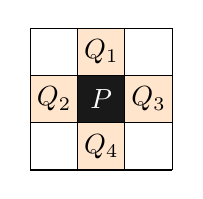
\begin{tikzpicture}[scale=0.6]
                \draw (0,0) grid (3,3);
                \filldraw[fill=orange!20] (1,0) rectangle (2,1);
                \filldraw[fill=orange!20] (1,2) rectangle (2,3);
                \filldraw[fill=orange!20] (0,1) rectangle (1,2);
                \filldraw[fill=orange!20] (2,1) rectangle (3,2);
                \filldraw[fill=black!90] (1,1) rectangle (2,2);


                \node[white] at (1.5,1.5) {$P$};
                \node at (1.5,2.5) {$Q_1$};
                \node at (0.5,1.5) {$Q_2$};
                \node at (2.5,1.5) {$Q_3$};
                \node at (1.5,0.5) {$Q_4$};




            \end{tikzpicture}
            \caption{4-adjacency}
            \label{fig:a_4}
        \end{subfigure}%
        \begin{subfigure}{0.40\textwidth}
            \centering
            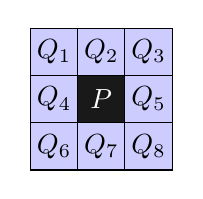
\begin{tikzpicture}[scale=0.6]
                \draw (0,0) grid (3,3);
                \filldraw[fill=blue!20] (0,3) rectangle (1,2);
                \filldraw[fill=blue!20] (2,0) rectangle (3,1);
                \filldraw[fill=blue!20] (0,0) rectangle (1,1);
                \filldraw[fill=blue!20] (2,2) rectangle (3,3);
                \filldraw[fill=blue!20] (1,0) rectangle (2,1);
                \filldraw[fill=blue!20] (1,2) rectangle (2,3);
                \filldraw[fill=blue!20] (0,1) rectangle (1,2);
                \filldraw[fill=blue!20] (2,1) rectangle (3,2);
                \filldraw[fill=black!90] (1,1) rectangle (2,2);
                \node[white] at (1.5,1.5) {$P$};
                \node at (0.5,0.5) {$Q_6$};
                \node at (1.5,0.5) {$Q_7$};
                \node at (2.5,0.5) {$Q_8$};
                \node at (0.5,1.5) {$Q_4$};
                \node at (2.5,1.5) {$Q_5$};
                \node at (0.5,2.5) {$Q_1$};
                \node at (1.5,2.5) {$Q_2$};
                \node at (2.5,2.5) {$Q_3$};
            \end{tikzpicture}
            \caption{$8-adjacency$}
            \label{fig:a_8}
        \end{subfigure}%

        \caption{3 different neighborhoods of pixel $P$ at location $(x,y)$.}
        \label{fig:adjacency}
    \end{figure}
\paragraph{Connectivity}
The connectivity of point $P$ is a set of points that can be reached in $n$ steps with a given adjacency type and intensity set $V$. If point $P$ is connected with $Q$ then there exist a path (or curve) from $P$ to $Q$ that consists of a sequence of distinct pixels with coordinates 
\begin{equation*}
    (x_0,y_0),(x_1,y_1),...,(x_n,y_n), \text{ where $n$ is the lenght of the path.}
\end{equation*}
If the path is closed then $(x_0,y_0) = (x_n,y_n)$
\paragraph{Region}
Let's define $R$ as an subset of pixels in an image. $R$ is a region if all points $\in R$ are a connected set, meaning that all points in $R$ are connected with each other and therefore form a region. This does not mean that the path connecting all points is closed.  Two regions can be adjacent to each other, if their union again forms a connected set. 

\paragraph{Boundary}
The outer boundary of a region $R$ is the set of pixels not in $R$ that are adjacent to pixels in $R$. In the definition of a boundary, the adjacency type is important. As a rule of thumb to define the boundary, the 8-adjacency is used. One important property of the outer boundary is, that it is a closed path. The inner boundary is the set of pixels that are in $R$ but are adjacent to at least one pixel that is not in $R$ and again the 8-adjacency is used. The inner boundary is not a closed path. 

\begin{figure}[ht]
    \centering
    \begin{subfigure}{0.40\textwidth}
        \centering
        \begin{tikzpicture}
            \matrix [matrix of nodes, nodes in empty cells, nodes={minimum width=1.5em, minimum height=1.5em, draw, thick, anchor=center}, column sep=-\pgflinewidth, row sep=-\pgflinewidth] (M)
            {
                |[fill=gray!20]| & |[fill=gray!20]| & |[fill=gray!20]| & |[fill=gray!20]| & |[fill=gray!20]| & |[fill=gray!20]| & |[fill=gray!20]| \\
                |[fill=gray!20]| & |[fill=gray!20]| & |[fill=gray!20]| & |[fill=red!20]|1 & |[fill=red!20]|1 & |[fill=gray!20]| & |[fill=gray!20]| \\
                |[fill=gray!20]| & |[fill=gray!20]| & |[fill=gray!20]| & |[fill=gray!20]| & |[fill=red!20]|1 & |[fill=red!20]|1 & |[fill=gray!20]| \\
                |[fill=gray!20]| & |[fill=gray!20]| & |[fill=gray!20]| & |[fill=gray!20]| & |[fill=gray!20]| & |[fill=red!20]|1 & |[fill=gray!20]| \\
                |[fill=gray!20]| & |[fill=red!20]|1 & |[fill=gray!20]| & |[fill=gray!20]| & |[fill=red!20]|1 & |[fill=red!20]|1 & |[fill=gray!20]| \\
                |[fill=gray!20]| & |[fill=red!20]|1 & |[fill=red!20]|1 & |[fill=red!20]|1 & |[fill=red!20]|1 & |[fill=gray!20]| & |[fill=gray!20]| \\
                |[fill=gray!20]| & |[fill=gray!20]| & |[fill=gray!20]| & |[fill=gray!20]| & |[fill=gray!20]| & |[fill=gray!20]| & |[fill=gray!20]| \\
            };
            
            \draw [thick] (M-1-1.north west) rectangle (M-7-7.south east);
        \end{tikzpicture}
        
        
            
        \caption{region $R$}
        \label{fig:region}
    \end{subfigure}%
    \begin{subfigure}{0.40\textwidth}
        \centering
        \begin{tikzpicture}
            \matrix [matrix of nodes, nodes in empty cells, nodes={minimum width=1.5em, minimum height=1.5em, draw, thick, anchor=center}, column sep=-\pgflinewidth, row sep=-\pgflinewidth] (M)
            {
                |[fill=gray!20]| & |[fill=gray!20]| & |[fill=red!20]| & |[fill=red!20]| & |[fill=red!20]| & |[fill=red!20]| & |[fill=gray!20]| \\
                |[fill=gray!20]| & |[fill=gray!20]| & |[fill=red!20]| & 1 & 1 & |[fill=red!20]| & |[fill=red!20]| \\
                |[fill=gray!20]| & |[fill=gray!20]| & |[fill=red!20]| & |[fill=red!20]| & 1 & 1 & |[fill=red!20]| \\
                |[fill=red!20]| & |[fill=red!20]|& |[fill=red!20]| & |[fill=red!20]| & |[fill=red!20]| & 1 & |[fill=red!20]| \\
                |[fill=red!20]| & 1 & |[fill=red!20]| & |[fill=red!20]| & 1 & 1 & |[fill=red!20]| \\
                |[fill=red!20]| & 1 & 1 & 1 & 1 & |[fill=red!20]| & |[fill=red!20]| \\
                |[fill=red!20]| & |[fill=red!20]| & |[fill=red!20]| & |[fill=red!20]| & |[fill=red!20]| & |[fill=red!20]| & |[fill=gray!20]| \\
            };
        
            \draw [thick] (M-1-1.north west) rectangle (M-7-7.south east);
        \end{tikzpicture}
        
        \caption{outer boundary (8-adjacent)}
        \label{fig:boundary}
    \end{subfigure}%
    \caption{Region and outer border.}
    \label{fig:regbond}
\end{figure}
\subsection{Preprocessing}
To be able to compare the different approaches, it is important to define the used algorithms that lead to the wanted result. An image taken has to be preprocessed first. The idea behind this step is to create a common ground for narrowing the deviation of the images down, so that the algorithms are able to recreate the same result over span of different images.
\subsubsection{Converting to grayscale}
As already presented in the previous chapter, the only colorful part of the eye is the iris. But the color itself is of no interest for the detection. Therefore the frames are first converted to grayscale. This is done by converting the colors into a gray intensity value. During this chapter the grayscale images have certain properties: 

\begin{table}[h]
    \centering 
    \begin{minipage}{0.7\textwidth}
      \centering
      \begin{tabular}{|c|c|c|}
        \hline
        Scaling &  Shape & numpy array type \\
        \hline
        100\% & 640x480& unit8 \\
        50\% & 320x240 & unit8 \\
        25\% & 160x120 & unit8 \\
        12.5\% & 80x60 & unit8 \\
        6.25\% & 40x30 & unit8 \\
        \hline
      \end{tabular}
      \caption{Scaling of the frames used in this thesis.}
      \label{tab:resoluiton}
    \end{minipage}\hfill
\end{table}

It is important to note that these resolutions are resolutions are congruent with the resolutions used in the LPW paper \cite{LPW}. This is important for the comparison of the results.
When scaling an image there is always an image interpolation done to find the best approximation for the new intensity value $I$. The interpolation used in this thesis is the bilinear interpolation.\cite{bilinearinter} This is a linear interpolation in the x and y axis of the intensity values and solves equation \ref{eq:bilinear}. let $Q_{11}=(x_1,y_1)$, $Q_{12}=(x_1,y_2)$, $Q_{21}=(x_2,y_1)$ and $Q_{22}(x_2,y_2)$ be the four surrounding points. The intensity value $I$ at $(x,y)$ is then calculated by equation \ref{eq:bilinear}. The point P at $(x,y)$ is the point of interest. 

\begin{figure}[h]
    \centering

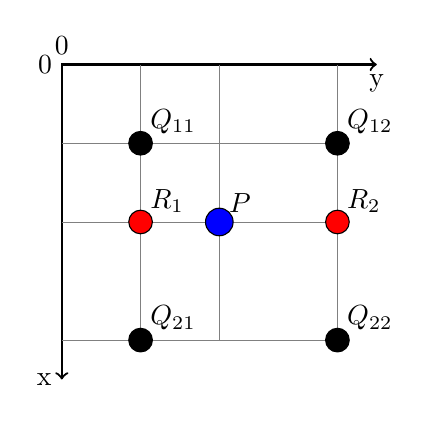
\begin{tikzpicture}[x=0.5cm,y=-0.5cm]
    
    % Draw the x-axis
    \draw[->,thick] (0,8) -- (0,0) -- (8,0) node[below] {y};
    % Draw the y-axis
    \draw[->,thick] (0,0) -- (0,8) node[left] {x};
    % Label the origin
    \node at (0,0) [left] {0};
    \node at (0,0) [above] {0};
    \foreach \x in {2,4,7}
    \draw[gray, very thin] (\x,0) -- (\x,7);
  \foreach \y in {2,4,7}
    \draw[gray, very thin] (0,\y) -- (7,\y);

    \foreach \Point/\PointLabel in {(7,4)/R_2,(2,4)/R_1}
    \draw[fill=red] \Point circle (0.3) node[above right] {$\PointLabel$};

    \foreach \Point/\PointLabel in {(2,2)/Q_{11}, (7,2)/Q_{12}, (2,7)/Q_{21}, (7,7)/Q_{22}}
    \draw[fill=black] \Point circle (0.3) node[above right] {$\PointLabel$};

    \foreach \Point/\PointLabel in {(4,4)/P }
    \draw[fill=blue] \Point circle (0.35) node[above right] {$\PointLabel$};

  \end{tikzpicture}

    \caption{Bilinear interpolation.}
    \label{fig:blinearInterpolation}
\end{figure}

\begin{minipage}{1\textwidth}
    \centering
    \begin{equation}
        v(x,y) = ax + by + cxy + d 
        \label{eq:bilinear}
    \end{equation}
    \begin{equation}
        f(R_{1}) \approx \frac{x_{2}-x}{x_{2}-x_{1}}f(Q_{11})+\frac{x-x_{1}}{x_{2}-x_{1}}f(Q_{21}) = R_{1}(x,y_{1})
    \end{equation}
    \begin{equation}
        f(R_{2}) \approx \frac{x_{2}-x}{x_{2}-x_{1}}f(Q_{12})+\frac{x-x_{1}}{x_{2}-x_{1}}f(Q_{22}) = R_{2}(x,y_{2})
    \end{equation}
    \begin{equation}
        f(P) \approx \frac{y_{2}-y}{y_{2}-y_{1}}f(R_{1})+ \frac{y-y_{1}}{y_{2}-y_{1}}f(R_{2}) = v(x,y)
    \end{equation}

    
\end{minipage}


\subsubsection{Histogram equalisation}
Another important aspect of preprocessing the frames is using Histogram equalization. This has the effect of increasing the contrast of the image. For this task Contras Limited Adaptive Histogram Equalization (CLAHE)\cite{clahe} is used. CLAHE is an Histogram Equalization method that has the benefit that it is adaptive to the local contrast of the image. This is very useful if the contrast of the image is not uniform. By using Histogram Equalization on the frames, noise is added to the image. This can be dealt with by using a low pass filter, like an Gaussian filter for example.

 Using a normal Histogram Equalization would lead to a loss of information in the region around the pupil and the iris. This is due to the fact that the contrast in this region is already very high. The CLAHE method splits the image into smaller blocks called "tiles"  and calculates the histogram on each block individualy and therefore does not lead to the same lose of important information at the pupil region. The CLAHE method is applied to the frames after they are converted to grayscale. The result of this step is shown in figure \ref{fig:clahe}. 

\begin{figure}[h]
    \centering
    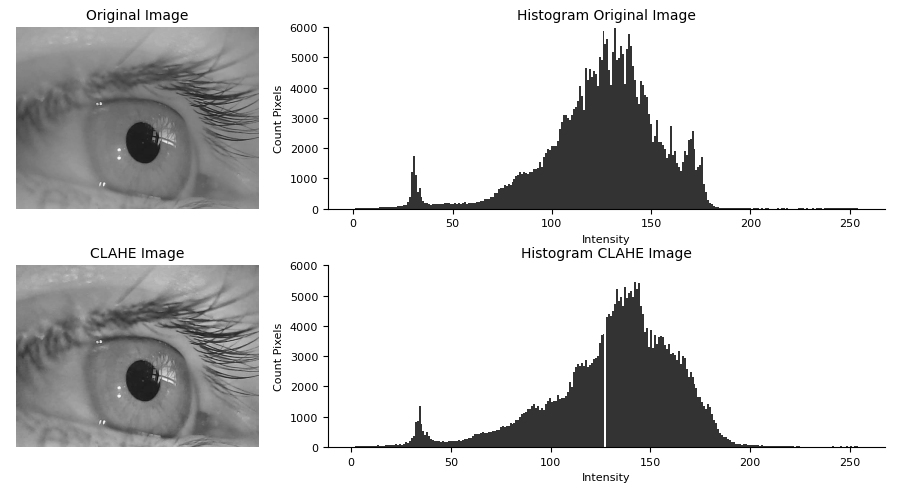
\includegraphics[width=1\textwidth]{plots/clahe.png}
    \caption{Example of CLAHE an its effect on the histogram.}
    \label{fig:clahe}
\end{figure}
These are the parameters used for the CLAHE plots
\begin{python}
    clahe = cv2.createCLAHE(clipLimit=1.0, tileGridSize=(11,11))
\end{python}

\subsection{Edge Detection}
The main goal behind edge detection is to find edges in the image. An edge is defined as a region that has a high contrast to its surrounding pixels, in other words a rapidly changing intensity in a small area. The edge detection is useful to filter the image for possible pupil contours. The edge detection analysis the image based on the change of intensity. Therefore a gradient calculation is used. There are different methods to calculate the gradient of an image. One of the most popular methods is the Sobel operator that makes use of the first differential of the image. The laplacian operator is another method that uses the second differential of the image. In this thesis the Sobel operator is used to calculate the gradient of the image. 
After calculating the gradient Canny edge detection is used to refine the edges. Canny edge detection is a multi step algorithm that uses a hysteresis thresholding to filter the edges. The result of the edge detection is a on pixel thick binary edge map.  All edges are now possible candidates for the pupil contour. 
\subsubsection{Sobel Operators}
The Sobel Operators are used is a common algorithm for edge detection. It is a gradient calculation that uses a 3x3 differential kernel to calculate the gradient of the image. The Sobel gradient is calculated in x and y direction. The gradient in x and y direction are calculated by convolving the image with two different kernels. The image with gray values is defined as $f(x,y)$ and the kernels are defined as $k_x$ and $k_y$. Therefore the gradient is calculated as follows:
\begin{equation}
    \nabla f = \begin{bmatrix}
        G_x \\ G_y
    \end{bmatrix} = \begin{bmatrix}
        \frac{\partial f}{\partial x}  \\ \frac{\partial f}{\partial y}
    \end{bmatrix}
\end{equation}

\begin{center}
    \begin{minipage}{0.44\textwidth}
        \begin{equation}
            k_x = \begin{bmatrix}
                -1 & 0 & +1 \\
                -2 & 0 & +2 \\
                -1 & 0 & +1
            \end{bmatrix} 
        \end{equation}
    \end{minipage}
    \hfill
    \begin{minipage}{0.44\textwidth}
        \begin{equation}
            k_y = \begin{bmatrix}
                -1 & -2 & -1 \\
                0 & 0 & 0 \\
                +1 & +2 & +1
            \end{bmatrix} 
        \end{equation}
         
    \end{minipage}
\end{center}

    \begin{align}
        G_x(x,y) & = f(x,y) * k_x  = \sum_{s=-a}^{a} \sum_{t=-b}^{b} k_x(s,t) f(x+s,y+t) \\
        G_y(x,y) & = f(x,y) * k_y  = \sum_{s=-a}^{a} \sum_{t=-b}^{b} k_y(s,t) f(x+s,y+t)
    \end{align}

    $G_x(x,y)$ and $G_y(x,y)$ are the gradients in x and y direction. $f(x,y)$ is the image and $k_x$ and $k_y$ are the kernels. The kernels convolved with the image $f(x,y)$ and the result is the gradient magnitude in x and y direction. In other words the convolution of an image with $k_x$ or $k_y$ gives as result the change from pixel to pixel in x or y direction.
    In python the Sobel in x and y are calculated with the OpenCV Library for example:

    \begin{python}
    G_x = cv2.Sobel(img,cv2.CV_64F,1,0,ksize=3)
    G_y = cv2.Sobel(img,cv2.CV_64F,0,1,ksize=3)
    \end{python}
    The total gradient magnitude $G$ is calculated with this equation: 
    \begin{equation}
        G = \sqrt{G_x^2 + G_y^2}
        \label{eq:gradientmagnitude}
    \end{equation} 
    and the direction $\theta$ of the gradient is calculated with this equation:
    \begin{equation}
        \theta = \arctan{\frac{G_y}{G_x}}
        \label{eq:gradientdirection}
    \end{equation}
    The result of the convolution can be seen in figure \ref{fig:gradient} in chapter two. 

    \subsubsection{Canny Edge Detection} 
    The Canny Edge Detection is used to recieve single edge points form the gradient magnitude image.  
    This algorithm can summarized in four steps\cite{canny_edge}: 
    \begin{enumerate}
        \item Noise reduction, smoothing the image with a Gaussian filter
        \item Compute the gradient magnitude and direction
        \item Non-maximum suppression to the gradient magnitude image
        \item Use double thresholding and connectivity analysis to detect and link edges
    \end{enumerate}
\textbf{Step 1: Noise reduction} \\
The first step is to reduce noise from the input image. This is done by convolving the image with a low pass filter. For this task a Gaussian filter is used. The Gaussian filter is defined as:
\begin{equation}
    f_{filter}(x,y) = \frac{1}{2\pi\sigma^2}e^{-\frac{x^2+y^2}{2\sigma^2}}
\end{equation}
The Gaussian filter is then convolved with the image so smooth the image. 
\begin{equation}
    f_{smoothed}(x,y) = f(x,y) * f_{filter}(x,y)
\end{equation} 

\textbf{Step 2: Compute the gradient magnitude and direction} \\
The gradient magnitude is calculated with the equation \ref{eq:gradientmagnitude} and the gradient direction is calculated with the equation \ref{eq:gradientdirection}.

\textbf{Step 3: Non-maximum suppression} \\
The non-maximum suppression is used to thin the edges out, so that the edges are only one pixel wide. This can be achieved with an loop that goes over all edges and checks if the current pixel, belonging to the edge, is the local maximum in the direction of the $\pm $gradient vector. If that is the case the pixel is kept, otherwise it is set to zero. Because as already described in \ref{subsec:funda} the coordinate system is defined different. The gradient direction is in reference to the $x$ axis. 



\begin{figure}[h]
    \centering
        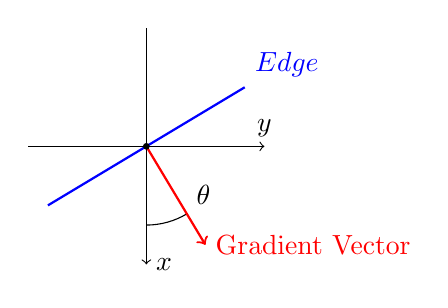
\begin{tikzpicture}[rotate=-90, scale= 0.5]
            % Draw the coordinate axes
            \draw[->] (-3,0) -- (3,0) node[right] {$x$};
            \draw[->] (0,-3) -- (0,3) node[above] {$y$};
            % Draw the first line
            \draw (2,0) arc (0:31:2)node[above right] {$\theta$};
            \draw[->,red,thick] (0,0) -- (2.5,1.5)node[right] {Gradient Vector};
            % Draw the angle marker
        
        ;
            % Draw the second line
            \draw[blue,thick] (1.5,-2.5) -- (-1.5,2.5)node[above right] {$Edge$};
            % Draw the origin
            \filldraw[black] (0,0) circle (2pt);
        \end{tikzpicture}
        \caption{Definition of the gradient direction}
        \label{fig:Definition_grad}
\end{figure}
Because an image is quantized, this also means that $\theta$ needs to be quantized to four directions to evaluate their neighbors. 

\begin{figure}[h]
    \centering
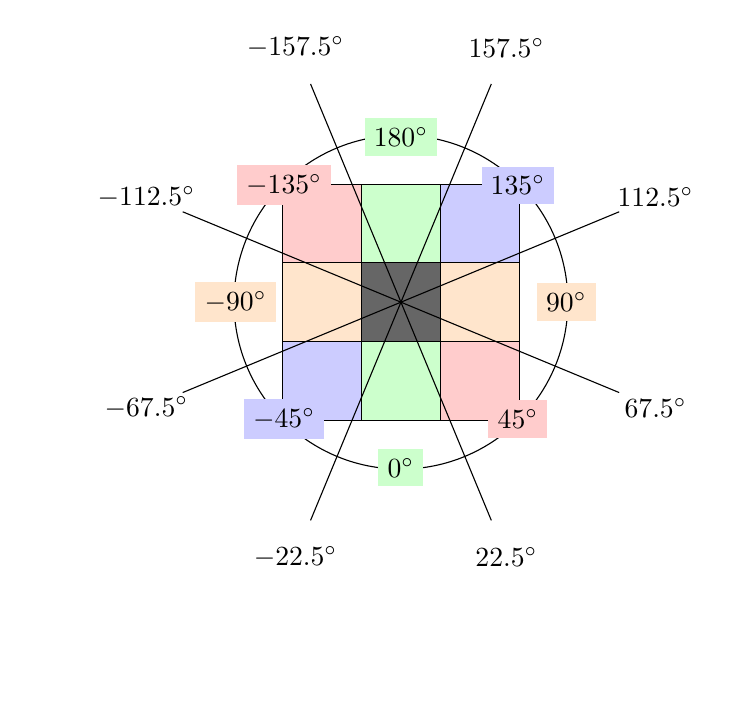
\begin{tikzpicture}[x=1cm,y=1cm]
    % Draw the grid
    \draw (0,0) grid (3,3);
     % Draw unit circle around grid

    % Fill the center pixel with light gray
    \filldraw[fill=blue!20] (0,0) rectangle (1,1);
    \filldraw[fill=blue!20] (2,2) rectangle (3,3);
    \filldraw[fill=orange!20] (0,1) rectangle (1,2);
    \filldraw[fill=orange!20] (2,1) rectangle (3,2);
    \filldraw[fill=red!20] (0,3) rectangle (1,2);
    \filldraw[fill=red!20] (2,0) rectangle (3,1);
    \filldraw[fill=green!20] (1,0) rectangle (2,1);
    \filldraw[fill=green!20] (1,2) rectangle (2,3);
    \filldraw[fill=black!60] (1,1) rectangle (2,2);


    \draw (1.5, 1.5) circle [radius=2.12];
    % Mark angles in 45° steps
    \foreach \ang in {157.5,112.5,67.5,22.5,-22.5,-67.5,-112.5,-157.5} {
        \draw (\ang-90:3.5) ++(1.5,1.5) node [fill=white] {$\ang^\circ$};
        \draw (\ang-90:3) ++(1.5,1.5) -- (1.5,1.5) ;

    }
    \foreach \ang in {0,180} {
        %\draw[thick,green] (\ang-90:2.3) ++(1.5,1.5) -- (1.5,1.5) ;
        \draw (\ang-90:2.1) ++(1.5,1.5) node [fill=green!20] {$\ang^\circ$};

    }

    \foreach \ang in {-45,135} {
        %\draw[thick,blue] (\ang-90:2.3) ++(1.5,1.5) -- (1.5,1.5) ;
        \draw (\ang-90:2.1) ++(1.5,1.5) node [fill=blue!20] {$\ang^\circ$};


    }
    \foreach \ang in {-90,90} {
        %\draw[thick,orange] (\ang-90:2.3) ++(1.5,1.5) -- (1.5,1.5) ;
        \draw (\ang-90:2.1) ++(1.5,1.5) node [fill=orange!20] {$\ang^\circ$};


    }
    \foreach \ang in {45,-135} {
        %\draw[thick,red] (\ang-90:2.3) ++(1.5,1.5) -- (1.5,1.5) ;
        \draw (\ang-90:2.1) ++(1.5,1.5) node [fill=red!20] {$\ang^\circ$};


    }

         % Add a tick at 45 degrees

\end{tikzpicture}
  \caption{Quantization of the gradient direction}
  \label{fig:non_max}
\end{figure}
This leads following quantizations: 
\begin{equation}
    \theta_q = \begin{cases}
    90, & \text{if } 67.5^\circ < \theta \leq 112.5^\circ \, \vee \, -112.5^\circ < \theta \leq -67.5^\circ \\
    -45^\circ, &\text{if }22.5^\circ < \theta \leq 67.5^\circ \, \vee \, -157.5^\circ < \theta \leq -112.5^\circ \\
    +45^\circ, &\text{if }112.5^\circ <\theta \leq 157.5^\circ \, \vee \, -67.5^\circ < \theta \leq -22.5^\circ \\
    0^\circ, &\text{if }-22.5^\circ <\theta \leq 22.5^\circ \, \vee \, -157.5^\circ < \theta \leq 157.5^\circ \\
\end{cases} 
\label{eq:quantization_d}
\end{equation}
It is important to note that when following the gradient direction, the two neighboring pixels are used to evaulate the gradient magnitute maximum. This is shown in figure \ref{fig:non_max} and \ref{fig:neighbors}.
If the gradient is maximal at the current pixel at $(x,y)$, meaning it is a local maximum in the previous defined neighborhood in respect to the gradient direction, the value of the pixel is written into $g_n(x,y)$, otherwise it is set to zero $g_n(x,y) = 0$. This is called non-maximum suppression. Therefore $g_n(x,y)$ contaians only the thinned edges.  

\begin{figure}[ht]
    \centering
    \begin{subfigure}[b]{0.23\textwidth}
        \centering
        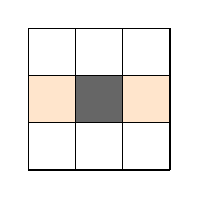
\begin{tikzpicture}[scale=0.6]
            \draw (0,0) grid (3,3);
            \filldraw[fill=orange!20] (0,1) rectangle (1,2);
            \filldraw[fill=orange!20] (2,1) rectangle (3,2);
            \filldraw[fill=black!60] (1,1) rectangle (2,2);
        \end{tikzpicture}
        \caption{Neighbors: 90°}
        \label{fig:n90}
    \end{subfigure}%
    \begin{subfigure}[b]{0.23\textwidth}
        \centering
        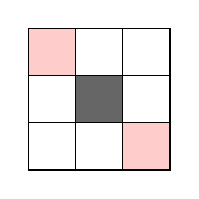
\begin{tikzpicture}[scale=0.6]
            \draw (0,0) grid (3,3);
            \filldraw[fill=red!20] (0,3) rectangle (1,2);
            \filldraw[fill=red!20] (2,0) rectangle (3,1);
            \filldraw[fill=black!60] (1,1) rectangle (2,2);
        \end{tikzpicture}
        \caption{Neighbors: 45°}
        \label{fig:n45}
    \end{subfigure}%
    \begin{subfigure}[b]{0.23\textwidth}
        \centering
        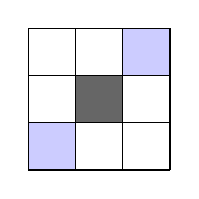
\begin{tikzpicture}[scale=0.6]
            \draw (0,0) grid (3,3);
            \filldraw[fill=blue!20] (0,0) rectangle (1,1);
            \filldraw[fill=blue!20] (2,2) rectangle (3,3);
            \filldraw[fill=black!60] (1,1) rectangle (2,2);
        \end{tikzpicture}
        \caption{Neighbors: -45°}
        \label{fig:nn45}
    \end{subfigure}%
    \begin{subfigure}[b]{0.23\textwidth}
        \centering
        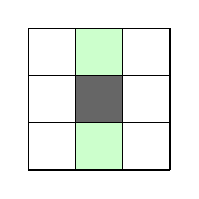
\begin{tikzpicture}[scale=0.6]
            \draw (0,0) grid (3,3);
            \filldraw[fill=green!20] (1,0) rectangle (2,1);
            \filldraw[fill=green!20] (1,2) rectangle (2,3);
            \filldraw[fill=black!60] (1,1) rectangle (2,2);
        \end{tikzpicture}
        \caption{Neighbors: 0°}
        \label{fig:n0}
    \end{subfigure}
    \caption{The gradient magnitude is evaluated in the direction of the gradient.}
    \label{fig:neighbors}
\end{figure}

  

\textbf{Step 4: Double thresholding and connectivity analysis} \\
After Step 3, $g_n(x,y)$ still shows edges that can be thicker than one pixel. $g_n(x,y)$ is then thresholded with a high an low threshold (hysteresis thresholding) creating two images: 
\begin{equation}
    g_{low}(x,y) = \begin{cases}
    g_n(x,y), & \text{if } g_n(x,y) \geq T_{low} \\
    0, &\text{otherwise}
\end{cases}
\end{equation}
\begin{equation}
    g_{high}(x,y) = \begin{cases}
    g_n(x,y), & \text{if } g_n(x,y) \geq T_{high} \\
    0, &\text{otherwise}
\end{cases}
\end{equation}
Because two different thresholds were used, there is still overlap between $g_{low}$ and $g_{high}$. All non zero pixels in $g_{high}$ are considered strong edge pixels. To recieve all weak edge pixels, the strong edge pixels are substracted from $g_{low}$. The remaining pixels are considered weak edge pixels.
\begin{equation}
    g_{weak}(x,y) = g_{low}(x,y) - g_{high}(x,y)
\end{equation}
Next step is to connect the weak edge pixels to the strong edge pixels. This is done by checking the 8-neighborhood of each strong edge pixel. If there is a weak edge pixel in the neighborhood, it is considered a strong edge pixel. This is done until no more weak edge pixels are found. The result is a binary image $g_{final}(x,y)$ containing all edges. But this still does not return a one pixel thick edge. 

To solve this the edges are passed on an edge-thinning algorithmus. Let's define the edges as set A and B as a structuring element. 
The equation for thining then becomes: 
\begin{equation}
    A \otimes   B = A - (A \circledast B)
\end{equation}
Where $\otimes$ is the thinning operator, $\circledast$ is the dilation operator.

\paragraph{Results}
In a frame where the pupil region clearly can be distinceted from the rest, the Canny edge detector can be used to find the pupil region. but as soon as more noise to the pupil is added, the hysteresis thresholding becomes more tricky and the detection accuracy decreases immensely. Also is it not possible to differentiate between the eye leashes, eye brows and the pupil. Therefore by using only the Canny edge detector. The pupil edges can not be found reliable and the algorithm itself is not adaptable to a great varriety of environments. 


\begin{figure}[ht]
    \centering
    \begin{subfigure}{.5\textwidth}
      \centering
      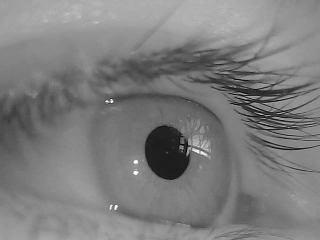
\includegraphics[width=.9\linewidth]{plots/orig_canny.png}
      \caption{Original image, scaling 0.5}
      \label{fig:orig_canny}
    \end{subfigure}%
    \begin{subfigure}{.5\textwidth}
      \centering
      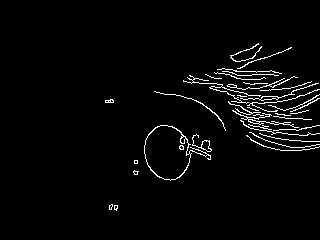
\includegraphics[width=.9\linewidth]{plots/canny.png}
      \caption{Clear pupil region, Canny edge detection}
      \label{fig:canny_region_clear}
    \end{subfigure}
    \caption{Canny edge detection on a clear pupil region}
    \label{fig:canny_clear}
\end{figure}

\begin{figure}[ht]
    \centering
    \begin{subfigure}{.5\textwidth}
      \centering
      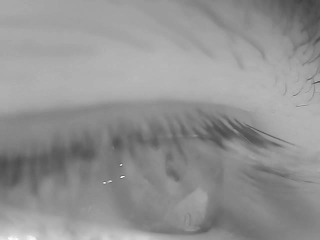
\includegraphics[width=.9\linewidth]{plots/orig_canny_eyelids.png}
      \caption{Original image, scaling 0.5}
      \label{fig:orig_canny_lids}
    \end{subfigure}%
    \begin{subfigure}{.5\textwidth}
      \centering
      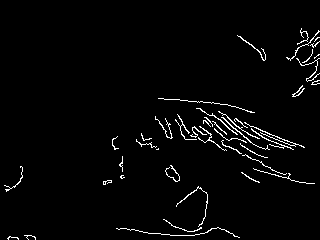
\includegraphics[width=.9\linewidth]{plots/canny_eyelids.png}
      \caption{Weak pupil region, Canny edge detection}
      \label{fig:canny_eyelid}
    \end{subfigure}
    \caption{Canny Edge detection on a frame with weak pupil region}
    \label{fig:canny_eyelid}
\end{figure}

\subsection{Haar like feature detection}
\subsubsection{Concept}
Haar like features is based on the observation that object have a certain local intensity variation in an image and this fact can be useful to identify objects. Haar like features makes use of this and divides the image into rectangular regions and then calculates the difference between the sum of the pixels in the white and gray regions, show in figure \ref{fig:haar_features}. This is done for all possible rectangular positions in the image. The result is a feature vector that is used to classify the image and give insight about the position of the object. In theory the feature is convolved with the image to calculate the feature vector but to make the detection faster, the integral image is calculated once and then used to calculate the feature vector at each possible position in the image.
 This leads to an easy calculation of the feature vector than now only needs four values to be calculated. 
The properties of the different features bring different abilities to detect specific local intensity patterns that are an indicator for a certain object or image region property. 
\subsubsection{Features characteristics}
To get a better understanding of the different features and their characteristics of the resulting feature vector the four features are explained a little more in detail. 
\paragraph{}
\begin{figure}[h]
    \centering
    
    \begin{subfigure}{0.45\textwidth}
        \centering
        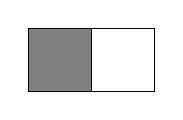
\begin{tikzpicture}[scale=0.8, transform shape]
            % Haar-like feature: Two-rectangle feature
            \draw[fill=gray] (0,0) rectangle (1,1);
            \draw[fill=white] (1,0) rectangle (2,1);
        \end{tikzpicture}
        \caption{Two-Rectangle Feature}
        \label{fig:haar_feature_1}
    \end{subfigure}
    \hfill
    \begin{subfigure}{0.45\textwidth}
        \centering
        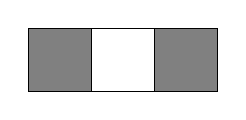
\begin{tikzpicture}[scale=0.8, transform shape]
            % Haar-like feature: Three-rectangle feature
            \draw[fill=gray] (0,0) rectangle (1,1);
            \draw[fill=white] (1,0) rectangle (2,1);
            \draw[fill=gray] (2,0) rectangle (3,1);
        \end{tikzpicture}
        \caption{Three-Rectangle Feature}
        \label{fig:haar_feature_2}
    \end{subfigure}
    
    \vspace{1.5em}
    
    \begin{subfigure}{0.45\textwidth}
        \centering
        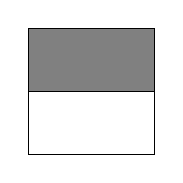
\begin{tikzpicture}[scale=0.8, transform shape]
            % Haar-like feature: Line feature (Horizontal)
            \draw[fill=gray] (0,0) rectangle (2,1);
            \draw[fill=white] (0,-1) rectangle (2,0);
        \end{tikzpicture}
        \caption{Horizontal Line Feature}
        \label{fig:haar_feature_3}
    \end{subfigure}
    \hfill
    \begin{subfigure}{0.45\textwidth}
        \centering
        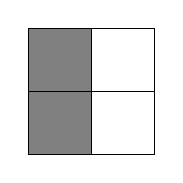
\begin{tikzpicture}[scale=0.8, transform shape]
            % Haar-like feature: Four-rectangle feature
            \draw[fill=gray] (0,0) rectangle (1,1);
            \draw[fill=white] (1,0) rectangle (2,1);
            \draw[fill=gray] (0,1) rectangle (1,2);
            \draw[fill=white] (1,1) rectangle (2,2);
        \end{tikzpicture}
        \caption{Four-Rectangle Feature}
        \label{fig:haar_feature_4}
    \end{subfigure}
    
    \caption{Haar-like Features}
    \label{fig:haar_features}
\end{figure}

The key concept to keep in mind is, that the features generate a response based on the difference of the sum of the pixels in the white and gray regions and therefore are able to detect local intensity patterns. The response of each feature also depends on the size of the feature and stands in relation to the size of the object that is to be detected. The result of the Haar-like features provides information about the presence or absence of a certain pattern that is reflected in the structure of the feature used. Because an object can have more than one fitting feature, the features are often used in a cascade of classifiers. The first classifier is a very simple classifier that is able to detect a lot of features. The following classifiers are more complex and are only used if the previous classifier was able to detect a certain feature. This leads to a very fast detection of the object. This safes computational resources and time. Often Machine learning is involved to classify if an object is present or not, based on the feature vectors. 

\subsubsection{Haar-Like Feature for pupil detection}
One very useful feature for finding a point in the pupil is given by a feature described in the paper \cite{pupil_haar}. This feature is constructed differently but used the same way as the other features to calculate an feature vector or response map. 
\begin{figure}
    \centering
    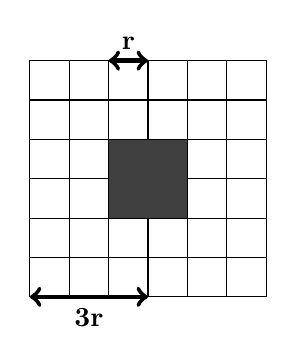
\begin{tikzpicture}[scale=0.5]

        % Grid
        \foreach \x in {0,1,...,5} {
            \foreach \y in {0,1,...,5} {
                \draw (\x,\y) rectangle ++(1,1);
            }
        }
    
        % Center 2x2 area
        \draw[fill=black!75] (2,2) rectangle ++(2,2);
        


       % Measurement on top
    \draw[<->, ultra thick] (0,0) -- (3,0) node[midway, below, font=\bfseries] {3r};

    % Measurement at the bottom
    \draw[<->, ultra thick] (2,6) -- (3,6) node[midway, above, font=\bfseries] {r};
    
    \end{tikzpicture}
\label{haar_pupil}
\caption{Haar-like feature for pupil detection}
\end{figure}


\subsection{Thresholding and Ellipse fitting}
\subsubsection{Thresholding}
In Thresholding the characteristic of the pupil is used, that it is the darkest part of the eye as seen in \ref{fig:hist1} . Here it is important to find a certain thresholding value to only extract the pupil. Considering the best scenario that the pupil is not affected by too much noise: no eyelash, no reflection. This method can be reliable to find the pupil region. This process shows to be less computation expensive and finds the pupil fast. 

The most difficult part is to find a fitting threshold value. This could be done by using the histogram of the frame. When inspecting the histogram, one could consider the lowest peak in the histogram as the given center value for thresholding. But this is not always the case. There is also the possibility for adaptive thresholding for example otsu thresholding. but throughout the work with thresholding otsu was also tested but was found to be less reliable than the histogram approach itself. 

\begin{figure}[ht]
    \centering
    \begin{subfigure}{.5\textwidth}
      \centering
      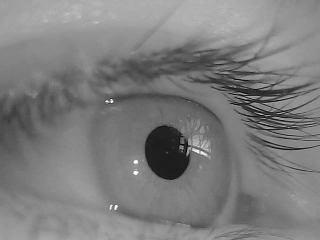
\includegraphics[width=.9\linewidth]{plots/orig_canny.png}
      \caption{Original frame}
      \label{fig:th_orig}
    \end{subfigure}%
    \begin{subfigure}{.5\textwidth}
      \centering
      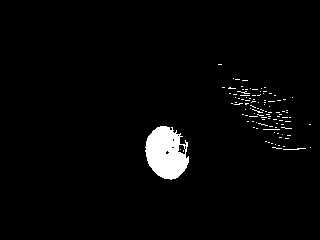
\includegraphics[width=.9\linewidth]{plots/thresholded.jpg}
      \caption{thresholded frame}
      \label{fig:th_thres}
    \end{subfigure}
    \caption{Original and thresholded frame}
    \label{fig:simple_thresh}
\end{figure}
in \ref{fig:simple_thresh} it can be seen that the thresholding is extremely volatile to reflections, eyelashes and other noise. This is why thresholding only has a good performance in a strictly defined environment with almost no noise. 

To showcase the volatility and the dependency on the threshold value, in \ref{fig:thresholded_images} a series of the same frame is shown with different threshold values (Th). It can be seen that the threshold value has to be chosen very carefully. If the value is chosen to low, the pupil region is not found. If the value is chosen to high, the much information is extracted and the pupil region can not be differentiated from the rest. 


\begin{figure}[htbp]
    \centering
    \begin{tabular}{cccc}
    \begin{subfigure}{0.2\linewidth}
    \centering
    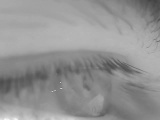
\includegraphics[width=\linewidth]{plots/thresholding/thresholded_eyelid.jpg}
    \caption{Original}
    \end{subfigure} &
    \begin{subfigure}{0.2\linewidth}
    \centering
    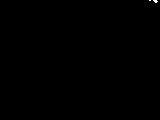
\includegraphics[width=\linewidth]{plots/thresholding/th1}
    \caption{Th = 65}
    \end{subfigure} &
    \begin{subfigure}{0.2\linewidth}
    \centering
    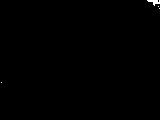
\includegraphics[width=\linewidth]{plots/thresholding/th2}
    \caption{Th = 71}
    \end{subfigure} &
    \begin{subfigure}{0.2\linewidth}
    \centering
    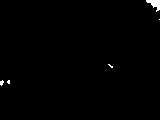
\includegraphics[width=\linewidth]{plots/thresholding/th3}
    \caption{Th = 77}
    \end{subfigure} \\
    \begin{subfigure}{0.2\linewidth}
    \centering
    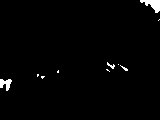
\includegraphics[width=\linewidth]{plots/thresholding/th4}
    \caption{Th = 83}
    \end{subfigure} &
    \begin{subfigure}{0.2\linewidth}
    \centering
    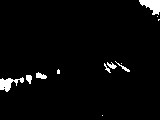
\includegraphics[width=\linewidth]{plots/thresholding/th5}
    \caption{Th = 89}
    \end{subfigure} &
    \begin{subfigure}{0.2\linewidth}
    \centering
    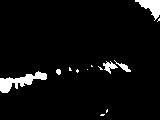
\includegraphics[width=\linewidth]{plots/thresholding/th6}
    \caption{Th = 95}
    \end{subfigure} &
    \begin{subfigure}{0.2\linewidth}
    \centering
    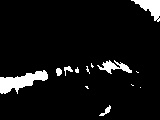
\includegraphics[width=\linewidth]{plots/thresholding/th7}
    \caption{Th = 101}
    \end{subfigure} \\
    \begin{subfigure}{0.2\linewidth}
    \centering
    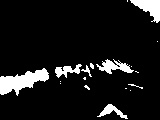
\includegraphics[width=\linewidth]{plots/thresholding/th8}
    \caption{Th = 107}
    \end{subfigure} &
    \begin{subfigure}{0.2\linewidth}
    \centering
    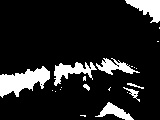
\includegraphics[width=\linewidth]{plots/thresholding/th9}
    \caption{Th = 113}
    \end{subfigure} &
    \begin{subfigure}{0.2\linewidth}
    \centering
    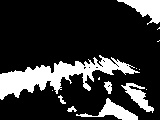
\includegraphics[width=\linewidth]{plots/thresholding/th10}
    \caption{Th = 119}
    \end{subfigure} &
    \begin{subfigure}{0.2\linewidth}
    \centering
    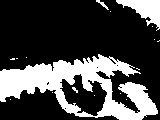
\includegraphics[width=\linewidth]{plots/thresholding/th11}
    \caption{Th = 125}
    \end{subfigure} \\
    \begin{subfigure}{0.2\linewidth}
    \centering
    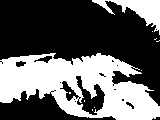
\includegraphics[width=\linewidth]{plots/thresholding/th12}
    \caption{Th = 131}
    \end{subfigure} &
    \begin{subfigure}{0.2\linewidth}
    \centering
    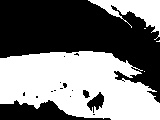
\includegraphics[width=\linewidth]{plots/thresholding/th13}
    \caption{Th = 137}
    \end{subfigure} &
    \begin{subfigure}{0.2\linewidth}
    \centering
    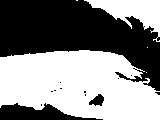
\includegraphics[width=\linewidth]{plots/thresholding/th14}
    \caption{Th = 143}
    \end{subfigure} &
    \begin{subfigure}{0.2\linewidth}
    \centering
    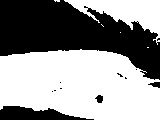
\includegraphics[width=\linewidth]{plots/thresholding/th15}
    \caption{Th = 149}
    \end{subfigure} \\
    \end{tabular}
    \caption{Thresholded images}
    \label{fig:thresholded_images}
    \end{figure}

    \subsubsection{Ellipse fitting}
    Ellipse fitting is based on finding a contour and fit an ellipse to it. The accuracy of the ellipse fit is strongly dependent on the quality of the contour extracted. The goal is to find the pupil as a connected region and than use ellipse fit to reconstruct the pupil as an ellipse. This involves solving equations with an approximation algorithm. For example least squares fitting. The least squares fitting is a method to find the best possible fit based on a set of data points. In this case points on the contour. The least squares fitting then calculated the distance from the possible ellipse curve to all points and minimizes the distance to all points. This is done by solving the following equations: 


 The general equation for an ellipse with center $(x_c, y_c)$, major axis $a$ and minor axis $b$ is:
\begin{equation}
    \frac{(x-x_c)^2}{a^2} + \frac{(y-y_c)^2}{b^2} = 1 
\end{equation}



To find all the values there is a need for at least 5 points on the contour of an possible ellipse. 
\begin{equation}
    J(a, b, x_c, y_c) = \sum_{i=1}^n \left(\frac{(x_i-x_c)^2}{a^2} + \frac{(y_i-y_c)^2}{b^2} - 1\right)^2
\end{equation}

where $n$ is the number of data points. The goal is to find the values of $a$, $b$, $x_c$, and $y_c$ that minimize this cost function.

We can use calculus to find the values of $a$, $b$, $x_c$, and $y_c$ that minimize $J$. The partial derivatives of $J$ with respect to $a$, $b$, $x_c$, and $y_c$ are:
\begin{equation}
\frac{\partial J}{\partial a} = 4\sum_{i=1}^n \frac{(x_i-x_c)^2}{a^3}\left(\frac{(x_i-x_c)^2}{a^2} + \frac{(y_i-y_c)^2}{b^2} - 1\right)
\end{equation}


\begin{equation}
    \frac{\partial J}{\partial b} = 4\sum_{i=1}^n \frac{(y_i-y_c)^2}{b^3}\left(\frac{(x_i-x_c)^2}{a^2} + \frac{(y_i-y_c)^2}{b^2} - 1\right)
\end{equation}

\begin{equation}
\frac{\partial J}{\partial x_c} = -8\sum_{i=1}^n \frac{x_i-x_c}{a^2}\left(\frac{(x_i-x_c)^2}{a^2} + \frac{(y_i-y_c)^2}{b^2} - 1\right)
\end{equation}

\begin{equation}
    \frac{\partial J}{\partial y_c} = -8\sum_{i=1}^n \frac{y_i-y_c}{b^2}\left(\frac{(x_i-x_c)^2}{a^2} + \frac{(y_i-y_c)^2}{b^2} - 1\right)
\end{equation}


We can set these partial derivatives to zero and solve for $a$, $b$, $x_c$, and $y_c$ to find the values that minimize $J$. This can be done using numerical methods such as Newton's method or gradient descent.

Once we have the values of $a$, $b$, $x_c$, and $y_c$, we can use the equation for an ellipse to draw the fitted ellipse on the data points.

Least square ellipse fitting is commonly used in image processing, computer vision, and pattern recognition to extract features from objects that can be approximated by ellipses, such as eyes, faces, or particles. When solving for the five different parameters, using the conic way described as: 
\begin{equation}
    Ax^2+Bxy+Cy^2+Dx+Ey+F=0
\end{equation}
    defining an ellipse if this condition is satisfied:
\begin{equation}
    B^2-4AC < 0
\end{equation}
or if using the parametric was described as: 
\begin{equation}
    (x-h)^2/a^2 + (y-k)^2/b^2 = 1
\end{equation}
the solution the the least square problem becomes a non linear problem and needs some sort of approximation. Depending on the kind of approximation different ellipses will be calculated. Also important to keep in mind, the ellipses are multiplied with an rotation matrix $R$ to fit the ellipse also to rotated ellipses. 
\begin{equation}
    R = \begin{bmatrix}
        \cos(\theta) & -\sin(\theta) \\
        \sin(\theta) & \cos(\theta) \\
    \end{bmatrix}
\end{equation}
    
\subsubsection{Contours}
    When working with thresholds the contour is of interests. The contour is defined as the outer boundary of the threshold binary matrix and is the foundation for the ellipse fit method. 
    Here it is not given to extract one single contour and therefore the contours need to be filtered based on which contour represents the pupil the best. 
    Mainly three criteria are used. 
    
    \paragraph{Circularity / Compactness}
    \begin{equation}
        \frac{4\pi\mathsf{A} }{()\oint_{\partial S} dS)^2}
    \end{equation}
    Where $\mathsf{A} $ is the Area of the contour, and it is devided by the integral over the outer boundary of the contour also known as the permitter of the contour.

    \paragraph{Similarity }
    The for the similarity the OpenCV library is used. This methods compares a given shape with another. As base for the comparison a simple ellipse is taken and then compared.

    \paragraph{Area}
    The Area of the contour should be maximal to find the greatest pupil area and filter out smaller area contours. 

   Each algorithm that returns a list of contours needs them to be checked with these four conditions and in the best case scenario only the contour of the pupil survives. This is then the contour on which a ellipse will be fitted. 


\subsection{Random Sample Consensus (RANSAC)}
The Random Sample Consensus (RANSAC) algorithm is an iterative method that is used to estimate the parameters for a known problem. For ellipse fitting a contour or a set of possible points inside or on the contour $C$ is the input. The algorithm then randomly selects a subset $S_c$ of 5 random selected points in $C$. 
These 5 points are then used to fit an ellipse as described in the section Ellipse Fitting.

\begin{figure}[h]
    \centering
    \begin{tikzpicture}[scale=0.4]
        % Drawing the coordinate system
        \draw[->] (-1,0) -- (12,0) node[right] {$x$}; % x-axis
        \draw[->] (0,-1) -- (0,12) node[above] {$y$}; % y-axis
        
        % Drawing the ellipse
        \draw[rotate around={30:(8,8)},scale=1] (8,8) ellipse (7cm and 5cm);
        
        % Annotations
        \node at (8,7) {$(h,k)$};
        \draw [rotate around={30:(8,8)},scale=1] (8,8) -- ++(7,0) node[midway,above] {$a$};
        \draw [rotate around={30:(8,8)},scale=1] (8,8) -- ++(0,5) node[midway,right] {$b$};
        \draw[scale=1, red] (8,8) -- ++(4.5,0) node[midway,above] {$\theta$};
        \draw[scale=1, red] (8,8) ++(4,0) arc (0:30:4);
        \filldraw[black] (8,8) circle (2pt);

    \end{tikzpicture}
    \caption{Ellipse with center $(h,k)$, semi-axes $a$ and $b$, and rotation $\theta$}
    \label{fig:sampleellipse}
\end{figure}

\begin{equation}
    \frac{((x-h)\cos(\theta) + (y-k)\sin(\theta))^2}{a^2} + \frac{((x-h)\sin(\theta) - (y-k)\cos(\theta))^2}{b^2} = 1
    \label{ellipsequation}
\end{equation}

The equation \ref{ellipsequation} represents an ellipse with major axis $a$, minor axis $b$ and the center of the ellipse at $(h,k)$. The angle $\theta$ is the rotation of the ellipse in the coordinate system. When comparing it with the general ellipse equation and compare coefficients the covariance matrix can be derived:
\begin{equation}
    \mathbf{A}x^2 + \mathbf{B}xy + \mathbf{C}y^2 = 1
    \label{ellipseco}
\end{equation} 
\begin{align}
    \mathbf{A}&=a^2 * \sin (\theta)^2 + b^2*\cos (\theta)^2 \\
    \mathbf{B}&= 2(b^2-a^2)*\sin (\theta)*\cos (\theta) \\
    \mathbf{C}&= a^2*\cos (\theta)^2 + b^2*\sin (\theta)^2
    \label{coefficients}
\end{align}
The covariance matrix is then defined as:

\begin{equation}
    \mathbf{V} = \begin{bmatrix}
        \mathbf{A} & \mathbf{B}/2 \\
        \mathbf{B}/2 & \mathbf{C} 
    \label{covariance}
    \end{bmatrix}
\end{equation}
The benefit of using the covariance matrix is, that the eigenvalues and eigenvectors have a direct relation to the major and minor axis and the rotation of the ellipse. The eigenvalues represent the major and minor of the axis and the eigenvectors represent the rotation matrix $R$ to rotate the ellipse in the coordinate system. This has the benefit that all parameters are known to transform all points into a new coordinate system where the calculated ellipse equation is represented in an unit circle.

\begin{figure}[h]
    \centering
    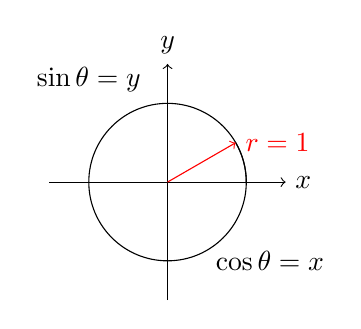
\begin{tikzpicture}
        % Draw the circle with radius 1
        \draw (0,0) circle (1);
        
        % Draw the axes
        \draw[->] (-1.5,0) -- (1.5,0) node[right] {$x$};
        \draw[->] (0,-1.5) -- (0,1.5) node[above] {$y$};
        
        % Define the angle
        \def\angle{30}
        
        % Draw the angle arc
        \draw (1,0) arc (0:\angle:1);
        
        % Draw the line and label
        \draw[->,red] (0,0) -- (\angle:1) node[right] {$r=1$};
        
        % Draw the labels for the trigonometric identities
        \node at (1.3,-1) {$\cos \theta = x$};
        \node at (-1,1.3) {$\sin \theta = y$};

    \end{tikzpicture}
    \caption{Unit circle with trigonometric identities}
    \label{fig:unit_circle}
\end{figure}

This allows for a simple distance calculation. Because $\lambda_{1,2}$ are known, the new coordsystem can be transformed to the unit circle by dividing the x and y values by the eigenvalues. The points form $C$ are then multiplied by the transposed eigenvectors to rotate the points into the new system and then divide by the eigenvalues. Let $p$ be a point in $C$ and $p'$ the transformed point in the new coordinate system. 
\begin{align}
    p' = R^T \begin{bmatrix} p_x - h \\ p_y - k \end{bmatrix} \odot \begin{bmatrix} \frac{1}{\lambda_1} \\ \frac{1}{\lambda_2} \end{bmatrix}\\
    r = \sqrt{p_x'^2 + p_y'^2}
    \label{distance calculation}
\end{align}
So the distance calculation of a point $p$ to the ellipse curve simplifies to the distance of the transformed point $p'$ to the unit circle.
\begin{equation}
    d = \sqrt{p_x'^2 + p_y'^2} -1
\end{equation}

By using this knowledge, the RANSAC algorithm iterates $n$ times to find the best ellipse with the most inliers. The inliers are calculated like following: 
\begin{equation}
    p =\begin{cases}
    \text{inlier} = \{p \in C | d < 0\}\\
    \text{border} = \{p \in C | d = 0\}\\
    \text{outlier} = \{p \in C | d > 0\}
    \end{cases}
    \label{inliers}
\end{equation}
The RANSAC algorithm calculates the ellipse parameters with five random points $S_c$ for $n$ iterations and evaluates each iteration the number of inliers. The ellipse with the most inliers is then used to calculate the final ellipse parameters with the best fit. 
The differentiation between on border an inlier is important to weight the focus on enclosing ellipses or on the border of the ellipse. Because the calculation of the distance $d$ is not an integer, it is possible that the distance is not exactly zero but still on the border. So it is important to keep in mind that comparing floats with each other, to alway use a small epsilon value that d can differ from 0 to set the threshold. 
In python functions like \textit{isclose} from the math module can be used to compare floats with each other. The number of iterations to find a 99\% chance of finding the best ellipse with the most inliers can be calculated with the following formula: 
\begin{equation}
    n = \frac{\log(1-p)}{\log(1-w^s)}
    \label{iterations}
\end{equation}
Where p = is the probability of finding the best ellipse and w is the ratio of inliers to outliers (Probability that a point is an inlier). This formula can then be used to estimate the number of iterations $n$ for the RANSAC algorithm to be 99\% sure to find the best ellipse with size $s$ as sample. In our case we use $s=5$, $p=0.99$ and for $w$ an approximation needs to be made. Because the number of inliers is unknown the ratio of inliers to outliers can not be calculated and needs to be estimated. In this case we assume that the ratio of inliers to outliers is $w=0.90$ which can be adapted later on. 
\begin{equation}
    n = \frac{\log(1-0.99)}{\log(1-0.90^5)} =  5.158
\end{equation}
So the number of iterations to find the best ellipse with the most inliers is 6. But it is important to keep in mind that this is only true if inliers are the sum of border and inliers. Otherwise the number of iterations needs to increase because the ratio inliers to outliers changes drastically. 

\subsection{Active Contouring}
Active contour segmentation is a method that is used to find the boundary curve of an object given that the object exists. There a many different approaches in active contouring but in this thesis two variants will be discussed. The first one being the classic classical snakes approach (Kass et al., 1988) with a simple energy function and the other variant being the active contouring without edges (ACWE) based on level sets. In both cases a initial contour is set and through iterative changes tries to find the boundary curve of an object. Each iteration the contour is changed by a small amount and then evaluated with an energy function. The energy function is a measurement of how well the contour is fitting to the edge of the object and in both cases the energy function is minimized.

Let $C(q): [0, 1] \rightarrow \mathbb{R}^2$ be a parametrized planar curve and let $I : [0, a] \times [0, b] \rightarrow \mathbb{R}^+$ be a given image used to detect the object boundaries with active contouring. The classical snakes approach (Kass et al., 1988) \ref{KASS} associates the curve $C$ with an energy given in \refeq{acgd}
But the most basic description for the energy minimization can be summarized in $E_{int}$ and $E_{ext}$ 
\begin{equation}
    E = E_{int} + E_{ext}
    \label{energy}
\end{equation}
\begin{equation}
        E(C) = \underbrace{\alpha \int_0^1 |C'(q)|^2 \, dq + \beta \int_0^1 |C''(q)|^2 \, dq}_{\text{E}_{int}} - \underbrace{\lambda \int_0^1 |\nabla I (C(q))| \, dq}_{\text{E}_{\text{ext}}}
\label{acgd}
\end{equation}
The goal is to minimize the energy function and by doing so the contour $C$ will find local minimals and depending on the sign of $lambda$ be attracted to light or dark edges. The first two terms of the energy describe the intern energy of the contour and the last term describes the external energy. In other words, the intern energy describes the curve smoothness and the external energy describes the relation of the curve to the edge at the curves boundary. In the following the three terms will be discussed in more detail.

To use these Equations, they have to be applied on a discrete grid. The curve $C$ is discretized into $N$ points  $c_i(x_i,y_i)$ with $i \in [0, N-1]$. The energy function is then calculated for each point $C_i$ and summed up to get the total energy of the curve. The energy function is then minimized by changing the position of the points $c_i(x_i,y_i)$ and the process is repeated until the energy function converges. The energy function is minimized by using the gradient descent method. The gradient of the energy function is calculated and the points $c_i(x_i,y_i)$ are changed by a small amount in the direction of the gradient. The gradient descent method is repeated until the energy function converge to a local minimal. 

The formula can be discretized by sampling the initial curve position evenly and then the formula can be expressed as following: 

\begin{equation}
    E = \sum_{i=0}^{N-1} \alpha (c_{i+1} - c_i)^2 + \beta (c_{i+2} - 2c_{i+1} + c_i)^2 - \lambda |\nabla I (c_i)|
\end{equation}
Here it is important to note, that the points are circular, when $i$ is equal to $N-1$ the next point is $c_0$. Therefore the indices can also be interpreted as $c_{(i+1 \bmod N)}$ and $c_{(i+2 \bmod N)}$
\begin{align*}
    \text {substitute:} \begin{cases}
    \sum_{i=0}^{N-1}(c_{i+1} - c_i) = C'(q) \\
    \sum_{i=0}^{N-1}(c_{i+2} - 2c_{i+1} + c_i) = C''(q)
    \end{cases}
\end{align*}

Where $C'(q)$ calculate the length of the curve and $C''(q)$ calculates the curvature of the curve.  

Because the classic snakes implementation searches for the best boundary curve that localy minimizes the energy function, the initial contour need to be initialized close to the best solution. Otherwise the algorithm will converge to a local minimum and not the global minimum. The classic snakes approach searches for the minimal with PDEs that is solved using the steepest descent method which brings performance issues and is prone to terminate early if a local minimum is found. 

\subsubsection{Active Contouring without Edges (ACWE)}
In ACWE the same principle is used to find the best object boundary. But in this case the energy function is minimized using level sets and morphological operations to solve the PDEs. \ref{muniz} The morphological operation use four different structuring elements. 

\begin{figure}[ht]
    \centering
    \begin{subfigure}[b]{0.23\textwidth}
        \centering
        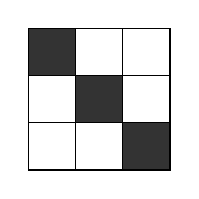
\begin{tikzpicture}[scale=0.6]
            \draw (0,0) grid (3,3);
            \filldraw[fill=black!80] (0,3) rectangle (1,2);
            \filldraw[fill=black!80] (2,0) rectangle (3,1);
            \filldraw[fill=black!80] (1,1) rectangle (2,2);
        \end{tikzpicture}
        \caption{Element 1}
        \label{fig:e1}
    \end{subfigure}%
    \begin{subfigure}[b]{0.23\textwidth}
        \centering
        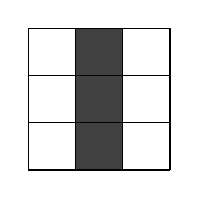
\begin{tikzpicture}[scale=0.6]
            \draw (0,0) grid (3,3);
            \filldraw[fill=black!75] (1,0) rectangle (2,1);
            \filldraw[fill=black!75] (1,2) rectangle (2,3);
            \filldraw[fill=black!75] (1,1) rectangle (2,2);
        \end{tikzpicture}
        \caption{Element 2}
        \label{fig:e2}
    \end{subfigure}
    \begin{subfigure}[b]{0.23\textwidth}
        \centering
        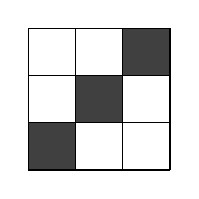
\begin{tikzpicture}[scale=0.6]
            \draw (0,0) grid (3,3);
            \filldraw[fill=black!75] (0,0) rectangle (1,1);
            \filldraw[fill=black!75] (2,2) rectangle (3,3);
            \filldraw[fill=black!75] (1,1) rectangle (2,2);
        \end{tikzpicture}
        \caption{Element 3}
        \label{fig:e3}
    \end{subfigure}%
    \begin{subfigure}[b]{0.23\textwidth}
        \centering
        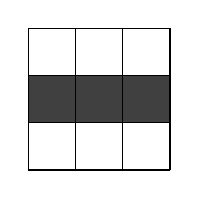
\begin{tikzpicture}[scale=0.6]
            \draw (0,0) grid (3,3);
            \filldraw[fill=black!75] (0,1) rectangle (1,2);
            \filldraw[fill=black!75] (2,1) rectangle (3,2);
            \filldraw[fill=black!75] (1,1) rectangle (2,2);
        \end{tikzpicture}
        \caption{Element 4}
        \label{fig:e4}
    \end{subfigure}%

    \caption{The four morphological structuring elements used in ACWE.}
    \label{fig:neighborsmorph}
\end{figure}
ACWE is based on Geodesic Active Contours (GAC). GAC has the benefit that it already solves key problems from the classical active contouring. Based on thresholds the contour is evaluated and decided if it flows expands the contour to a new pixel or not. GAC is based on classic active contours and geodesic curves in a Riemannian space. The level sets have the benefit that they can easily be implemented in a discrete grid and open the door to solve the PDEs using morphological operations. The level set approach brings more stability and is less sensitive to the initial contour compared to the classical active contouring method. It is also possible to detect the interior and exterior boundary. In the classical approach the interior force is based on first and second derivatives of the curve. This leads to stability, computational complexity and performance issues. This is solved in the GAC by using the evolution of an implicitly defined curve. The GAC algorithm based on a level set function $u$ is defined as following:
\begin{equation}
    \frac{\partial u}{\partial t} = 
    \underbrace{g(I) \cdot |\nabla u| \cdot \text{div} \left(\frac{\nabla u}{|\nabla u|}\right)}_{\text{Smoothing force}} 
    + \underbrace{g(I) \cdot \nu \cdot |\nabla u|}_{\text{Balloon force}} 
    + \underbrace{\nabla g(I) \cdot \nabla u}_{\text{External force}}.
    \label{deform}
    \end{equation}
    
Where $u$ is the level set function, a binary mask that is 1 inside the object and 0 outside. $I$ is the image, $g(I)$ is the edge indicator function, $\nu$ is a variable that decides in which direction and how strong the curve should move. 
For chosing $g(I)$ there are different variants but two of the most common are the following: 

\begin{align}
    g(I) = \begin{cases}
     \frac{1}{1 + |\nabla I|*\alpha} &(1)\\
     \\
     -|\nabla I| &(2)
    \end{cases}
\end{align}
In (1) $g(1)$ is low when the gradient is high and vice versa. Meaning that $g(I)$ regulates the influence of the forces depending on the gradient. It is around 0 when the gradient is high, in other words it stops the curve from moving when the the pixel has reached an edge. $\alpha$ is a variable that regulates how strong the influence of the external energy is.  In (2) $g(I)$ is negative when the gradient is high. So both definition of $g(I)$ will stop the curve from moving when it reaches an edge.

\paragraph{Smoothing force}
The smoothing force is the same as the curvature term in the classical snakes method. The difference is that in GAC the smoothing force is calculated using the gradient of the level set function $u$ instead of the curve. 
\begin{equation}
    g(I) \cdot |\nabla u| \cdot \text{div} \left(\frac{\nabla u}{|\nabla u|}\right)
\end{equation}
Now the smoothing force is calculated with using an recursive call of SI and IS of operator F that approximates the curvature flow that is based on PDE. 
\begin{equation}
    \text{F}(u) = SI(u)\circ IS (u)
    \label{eq:smoothingforce}
\end{equation}
Where SI means supremum of infimum and IS means infimum of supremum. In other words, SI stands for erode and IS stands for dilate. One step of smoothing looks like following: 
\begin{align*}
    1) u_{SI\circ IS}=\text{erode}(u) \circ \text{dilate}(u) \\
    2) u_{IS\circ SI}=\text{dilate}(u) \circ \text{erode}(u)
\end{align*}
by repeating step 1 to 2 the smoothing force can be stronger or weaker. But it is important so always use step 1 and step 2 in the same order. 


\paragraph{Balloon force}
The balloon force is important in regions where the gradient is low and hinders the curve flow to get stuck at a local minimum. Expecially when looking at the external force, where the velocity of the curve is determined by the gradient of $g(I)$ and the gradient of $u$. Ifh $g(I)$ goes to zero the curve will have no external velocity, therefore the balloon force is important to make the algorithm more robust.
\begin{equation}
    g(I) \cdot \nu \cdot |\nabla u|
\end{equation}
To make GAC more computational efficient the ballon force and also the smoothing force are computed differently. 
The Balloon force is $g(I)*|\nabla u| *v$ with parameter $v \in  {-1,1}$ can be substituted with dilation over the four different neighborhood structuring elements. Because dilation is a morphological operation it is computed very efficient and also gets rid of the PDEs that need to be solved in the classical snakes method. By using dialate the balloon force leads to the wanted result by making the curve grow. 
\begin{equation}
    \text{dialate}(u)  =  u \bigoplus Element_i \quad \text{for} \quad i \in \{1,2,3,4\}
    \label{dialate}
\end{equation}

\paragraph{External force}
The external force is the same as in the classical snakes method but in GAC it is weighted by $g(I)$ to stop the curve from moving when it reaches an edge.
\begin{equation}
    \nabla g(I) \cdot \nabla u
\end{equation}
The change in the level set function $u$ is only applied to the points where $g(I) > T$ where $T$ is a defined threshold to control the velocity and the characteristic that the curve moves faster in areas where the gradient is low. This leads to an algorithm that moves faster in a region with the same intensity and slower in regions with a high gradient. 
The external force or the attracting force is calculated for each point $p$ in the binary mask from the before modified level set function $u$ and evaluated with the following equation:
\begin{equation}
    p = \begin{cases}
        1 &iff  \nabla u * \nabla g(I) > 0 \\
        0 &iff \nabla u * \nabla g(I) < 0
    \end{cases}
    \label{eq:externalforce}
\end{equation}
\paragraph{Summary}
To conclude, the equation \refeq{eq:deform} describes the deformation of $u$, the binary level set function. and is the main equation for Geodesic Active Contours (GAC). 

\subsubsection{Convert GAC to ACWE}
The GAC only inspects places where the curve could move iteratively and this is the main difference to ACWE. ACWE also known as Chan-Vese algorithm takes the complete image into consideration to evaluate the boundary or the curvature flow of the level set. 
Let $c_i$ the the mean intensity of an subset $Oomega$ of the image $I$ and let $c_1$ be the mean intensity inside the curve or level set $u$ defined as $\Omega_1$ and $c_2$ the mean intensity outside level set $u$ defined as $\Omega_2$. 
\begin{equation}
    c_{i}= \frac{ \int_{\Omega_{i}} I(x) \,dx}{\int_{\Omega_{i}} \, dx }
\end{equation}
Then the external force function $F(c_1,c_2,C)$ can be defined as equation \refeq{eq_curvatureflow} where the first two terms $\mu \cdot \text{length}(u) + \nu \cdot |\text{inside}(u)|$ are the same as in the GAC The third and fourth terms sort of calculate the unscaled intensity variance in the different subsets $\Omega_1$ and $\Omega_2$. 
\begin{equation}
    \begin{split}
    F(c_1, c_2, C) = & \mu \cdot \text{length}(u) + \nu \cdot |\text{inside}(u)| \\
    & + \lambda_1 \cdot \int_{\Omega_1} (I(x) - c_1)^2 \, dx \\
    & + \lambda_2 \cdot \int_{\Omega_2} (I(x) - c_2)^2 \, dx
    \end{split}
    \label{curvatureflow}
    \end{equation}

Only difference now between the GAC and the ACWE is the external force that is calculated different. In GAC the external force is calculated with $\nabla g(I) \cdot \nabla u$ and considering if a point is inside or outside the curve based on a threshold as seen in equation \refeq{eq:externalforce}. In ACWE the external force is calculated with the mean intensity of the subsets $\Omega_1$ and $\Omega_2$ and the intensity of the image $I(x)$ as seen in equation \refeq{eq_curvatureflow}. Translating onto an discrete grid the equation can be written as: 
\begin{equation}
   \xi  = \underbrace{\lambda_{1} \cdot | \nabla u_{mask}| \cdot (I(x)-c_{1})^{2}}_{Inside}-\underbrace{\lambda_{2} \cdot|\nabla u_{mask}| \cdot (I(x)-c_{2})^{2}}_{outside}
\end{equation} 
$\xi$ is then used to calculate the new level set function $u$ with the following equation:
\begin{equation}
    u(x,y) = \begin{cases}
        1 \text{ if } \xi<0 \\
        0 \text{ if } \xi>0 \\
        \text{do nothing otherwise}
        \end{cases}
\end{equation}
The Gradient of the mask will only be nonzero at the contour of the mask. 
Now $I(x)$ is subtracted by the mean and each point on the contour will have two values, their inside and outside Intensities. By subtracting the mean intensity from the pixel intensities on the boundary of u, multiplying it with $\lambda_i$ and subtracting the outside term from the inside term an relationship between the inside and outside intensities is created and can be tuned with the sensitivity parameters $\lambda_i$ . This relationship is then used to calculate the new level set function $u$ and the process is repeated until the level set function converges. In a case where the function reaches the object boundary the inside and outside intensities will be the same and the curve will not move anymore. 
Here is an example of the evolution the the level set u when the ACWE algorithm is used with a given starting point inside the pupil. 
\begin{figure}[h]
    \centering
    \begin{subfigure}{0.3\textwidth}
        \centering
        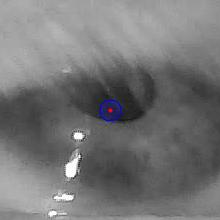
\includegraphics[width=0.9\linewidth]{plots/acwe/iteration_0.png}
        \caption{Initial level set}
    \end{subfigure}%
    \hfill
    \begin{subfigure}{0.3\textwidth}
        \centering
        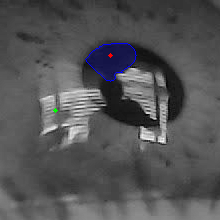
\includegraphics[width=0.9\linewidth]{plots/acwe/iteration_15.png}
        \caption{Iteration 15}
    \end{subfigure}%
    \hfill
    \begin{subfigure}{0.3\textwidth}
        \centering
        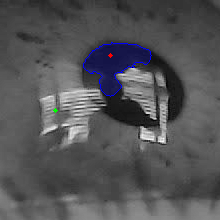
\includegraphics[width=0.9\linewidth]{plots/acwe/iteration_30.png}
        \caption{Iteration 30}
    \end{subfigure}%
    \hfill
    \begin{subfigure}{0.3\textwidth}
        \centering
        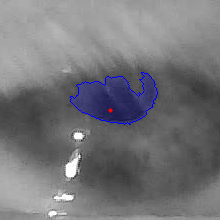
\includegraphics[width=0.9\linewidth]{plots/acwe/iteration_60.png}
        \caption{Iteration 60}
    \end{subfigure}
    \hfill
    \begin{subfigure}{0.3\textwidth}
        \centering
        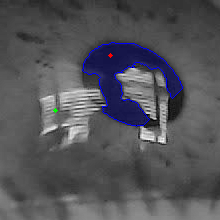
\includegraphics[width=0.9\linewidth]{plots/acwe/iteration_90.png}
        \caption{Iteration 90}
    \end{subfigure}
    \hfill
    \begin{subfigure}{0.3\textwidth}
        \centering
        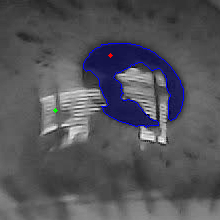
\includegraphics[width=0.9\linewidth]{plots/acwe/iteration_115.png}
        \caption{Iteration 115}
    \end{subfigure}
    \caption{ACWE iterations}
    \label{fig:iterations_acwe}
\end{figure}

\subsubsection{Active contouring with ellipse parameters}
A different approach is to use the let an ellipse grow and modify it's parameters based on the gradient information. By sampling an amount of equally spaced points on the ellipse and evaluate an energy function based on the image intensity gradient and the normal vector of the ellipse at those points. The energy function can be described as the scalar product of the gradient and the normal vector of the ellipse curve. 
\begin{equation}
    E = -\sum_{i=0}^{N-1} \nabla I \cdot \vec{n}
\end{equation} 
this converts the problem into a minimization problem. The energy function still needs a term to make sure that the curve grows and does not get stuck at a local minimum. Here it is not possible to use the morphological operators because the shape of the ellipse is not given as a level set. Instead is based on only the five ellipse parameter: center, axis, angle. 

\begin{figure}[h]
\centering
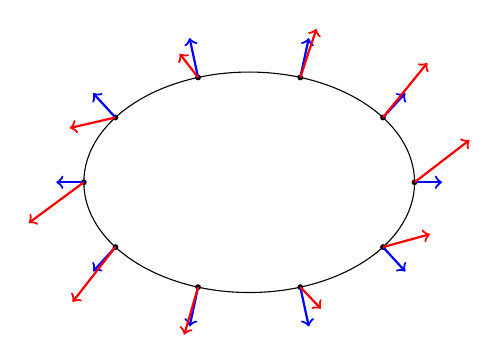
\begin{tikzpicture}[scale=0.7, transform shape]
    \def\a{3} % semi-major axis
    \def\b{2} % semi-minor axis
    \def\scale{1} % scale for normal and gradient vectors

    % Draw ellipse
    \draw (0,0) ellipse (\a cm and \b cm );
    
    % Draw 10 points and corresponding vectors
    \foreach \i in {1,2,...,10} {
        \pgfmathsetmacro{\angle}{\i*36}
        \pgfmathsetmacro{\xcoord}{\a*cos(\angle)}
        \pgfmathsetmacro{\ycoord}{\b*sin(\angle)}
        \coordinate (p\i) at (\xcoord,\ycoord);
        \fill (p\i) circle (1.5pt);

        % Normal vector
        \draw[->, blue, thick] (p\i) -- ++({\xcoord/\a^2*1.5*\scale},{\ycoord/\b^2*1.5*\scale});

        % Dummy gradient vector
        \draw[->, red, thick] (p\i) -- ++({\scale*cos(\angle+\i*0.5)},{\scale*sin(\angle+45+\i*0.5)});
    }
\end{tikzpicture}
\label{fig:normalgradientellipse}
\caption{Ellipse with normal vector (blue) and gradient vectors (red)}

\end{figure}
The energy function is the lowest when at each point the gradient vector and normal vector  point in the same direction. The gradient vector consists of the magnitude of the gradient and the orientation. Whereas the normal vector is normalized and points in the direction of the normal of the ellipse at that point. 

The problem with this approach is overlapping with the classical active contouring.  The initial contour needs to be close to the optimal solution. Otherwise the algorithm stops at an local minimum and convergence to the optimal solution is not guaranteed. Because it is an minimization with five parameters it is a very complex problem and the algorithm needs to be run multiple times to find the best local solution. Also the image needs strong preprocessing and the algorithm is very sensitive to noise. Therefore it is a must to first apply a low pass filter onto the image. But because of blurring the image gradients and directions aren't as accurate as the could be and struggles with reflections and other noise. Here is an example with the convergence to an local minimum. The initial ellipse is nowhere near to the optimal solution and the algorithm converges to an local minimum. 

\begin{figure}[h]
    \centering
    \begin{subfigure}{0.5\textwidth}
        \centering
        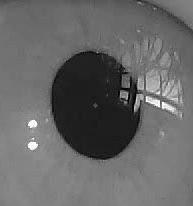
\includegraphics[width=0.7\linewidth]{plots/eye_dataset/roi.png}
        \caption{ROI}
    \end{subfigure}%
    \hfill
    \begin{subfigure}{0.5\textwidth}
        \centering
        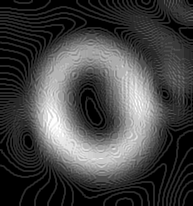
\includegraphics[width=0.7\linewidth]{plots/eye_dataset/mag.png}
        \caption{Gradient Magnitude}
    \end{subfigure}%
    \hfill
    \begin{subfigure}{0.5\textwidth}
        \centering
        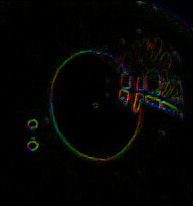
\includegraphics[width=0.7\linewidth]{plots/eye_dataset/direction.png}
        \caption{Gradient Direction}
    \end{subfigure}%
    \hfill
    \begin{subfigure}{0.5\textwidth}
        \centering
        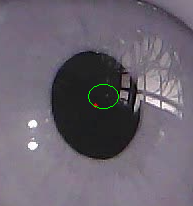
\includegraphics[width=0.7\linewidth]{plots/eye_dataset/result.png}
        \caption{Result}
    \end{subfigure}
    \caption{Convergence to local minimum}
    \label{fig:ac_ellipse_gradient}
\end{figure}
The problem with expanding the energy function with more terms is, that the algorithm gets more complex. For example when the size is used as a reward for the energy function (the bigger the better), it is not given anymore to stop at the boundary of the object. The parameters have to be chosen smart and carefully to make sure that the algorithm still converges to the optimal solution. 

\section{Results}
In this chapter some of the algorithm in the theory chapter are combined, tested and evaluated. The goal is to find the most robust combination of algorithms to detect the pupil even in a very demanding data set like the LPW. The LPW data set is already discussed in its chapter and will not be discussed here again. In general the evaluation can be split up into two part. The first part is localization of the pupil and second part is finding the pupil ellipse. The importance of the localization is that with the information of the location of the pupil it is possible to create a region of interest (ROI). This has the benefit that in the second part the image size is already decreased and additional noise can be even more limited. Also the computational effort is reduced because the image size is smaller. Important to note is, that all algorithms make the basic assumption, that the pupil is always visible. So blinking is not counted as a failure and excluded of the evaluation if possible. For detecting blinking, other algorithms need to be used to preprocess every frame and detect if the eye is closed or not. 


\subsection{Localization}
For the localization mainly thresholding, edge detection and haar-like features were implemented and can now be evaluated. To make thresholding more flexible a semi adaptive algorithm was created to choose the best fitting threshold value. The histogram is used to determine the highest peak in the low intensity range. This value is then used to threshold the image. 
\begin{equation}
    t = \text{argmax} \{h(i) | i \in [0,255]\}
\end{equation}
With $h(i)$ being the histogram of the image. The threshold value is then used to calculate a range for using double thresholding to extract the pupil. The image is modified by setting all values below and above the threshold value to 0. 
\begin{equation}
    f(x,y)= \begin{cases}
        0 &iff \quad I(x,y) < t-35 \quad \text{or} \quad I(x,y) > t+25 \\
        I(x,y) &otherwise
    \end{cases}
\end{equation}
\subsubsection{Thresholding}
Whereas the under limit of the threshold is set lower than the higher limit. This derives from testing and can be concluded, that the probability that the pixels with lower intensity values belongs to the pupil is higher than the probability that the pixels with higher intensity values belong to the pupil. In a environment with almost no noise and most important no reflections this approach works very well. But as also already mentioned in the theory section, reflections lead to a less higher peak in the histogram and the possibility exist that the threshold value has no peak in the lower values range and therefore leads to a faulty result that can not be used to create an ROI or use it with edge detection to find the boundary of the pupil. Also it is important to note that with this thresholding approach the mask created is not a binary mask but a mask with values between $[t-35, t+25]$. But the possibility to use the binary mask still exist and the all contours found in this threshold range are evaluated by their circularity and similarity to an ellipse. The best fitting contour is then used to create the ROI or ellipse fit directly to find the ellipse parameters. 
[RESULTS]
This method works in a environment with almost no noise flawless, it is has benefit to reach the goal in almost realtime but in with the LPW data set it is keen to strugle with most of the conditions and is therefore not usefull for the LPW data set.

\subsubsection{Edge detection}
Edge detection is strongly effected by noise and therefore the preprocessing is key for useful results. Every frame undergoes the same preprocessing as in the other algorithms but a gaussian blur is used additionally to smooth fast changing intensity regions out.  Even though the gaussian blur is used, there is still information missing that is covered by noise. The edges are detected but the same problem as with thresholding arises here. By using Sobel and than the Canny edge detection the results are useful in a environment with almost no noise but as already said, LPW is known for its noise and reflections. Canny edge detection needs two threshold parameters to work properly and also here arises the problem that these parameters need to be adaptive to the environment which can be tricky. 
[RESULTS]

\subsubsection{Haar-like features}
The Haar-like feature is the approach that is proposed by this thesis to find the region of interest. It has the best detection rate of all approaches tested on the LPW data set and is therefore the best approach to find the ROI. The Haar-like feature is constructed as described in the theory part and is shown in \ref{fig:haar_pupil}. 
The calculation of the feature vector is done by using the integral image and is done 3 times with variating Radius $r$ all feature vectors are then compared and the location of the highest response is returned as a point that lies on the pupil. 

\begin{figure}[h]
    \centering
    \begin{subfigure}{0.5\textwidth}
        \centering
        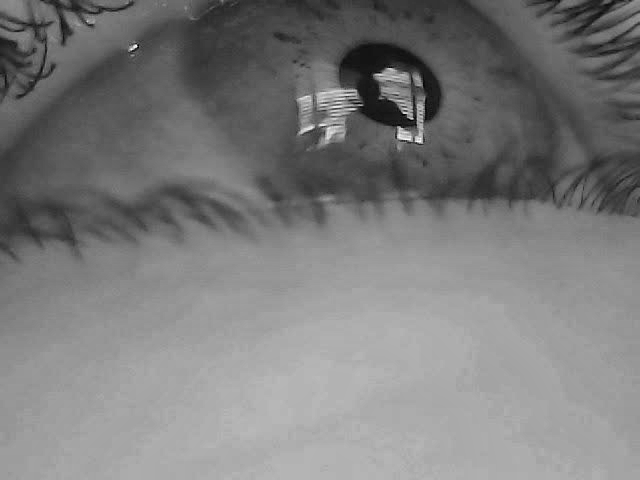
\includegraphics[width=0.9\linewidth]{plots/results/originalbest.png}
        \caption{Original Frame}
    \end{subfigure}%
    \hfill
    \begin{subfigure}{0.5\textwidth}
        \centering
        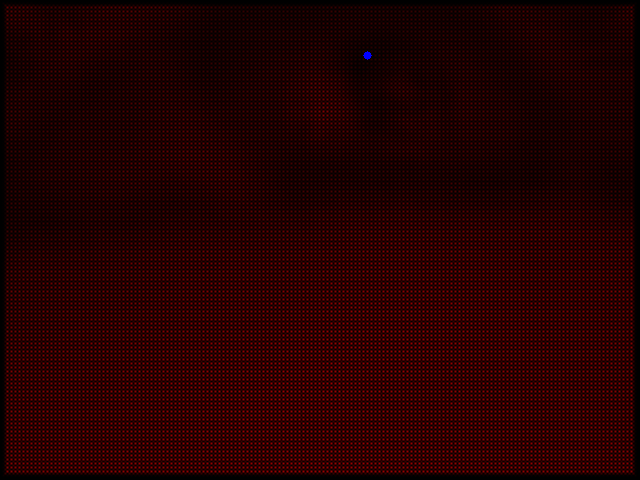
\includegraphics[width=0.9\linewidth]{plots/results/responsehaarbest.png}
        \caption{feature vector, blue is the best response}
    \end{subfigure}%
 
    \caption{Feature vector for pupil detection}
    \label{fig:limit_haar}
\end{figure}

The stronges response lies then within the pupil and the location is then used to create a ROI. In this case a ROI of $110 x 110$ was the norm but depending on the rescaling of the frames this can be adapted. Important to note is, that the returned point in the pupil is not given to be in the center. This in an important fact when choosing the size of the ROI that is created. 
But this approach is still not perfect and even though it can handle noise really good, there are limits to the amount of noise until the algorithm fails. Also the algorithm is not able to detect the pupil when the eye is closed.

\begin{figure}[h]
    \centering
    \begin{subfigure}{0.5\textwidth}
        \centering
        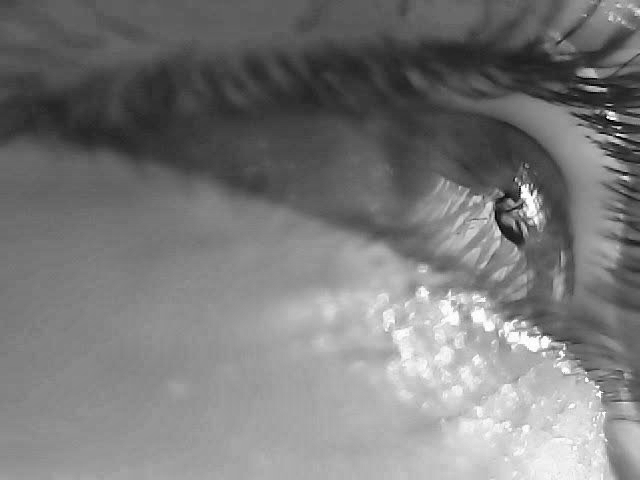
\includegraphics[width=0.9\linewidth]{plots/results/originalworst.png}
        \caption{Extreme noise example}
    \end{subfigure}%
    \hfill
    \begin{subfigure}{0.5\textwidth}
        \centering
        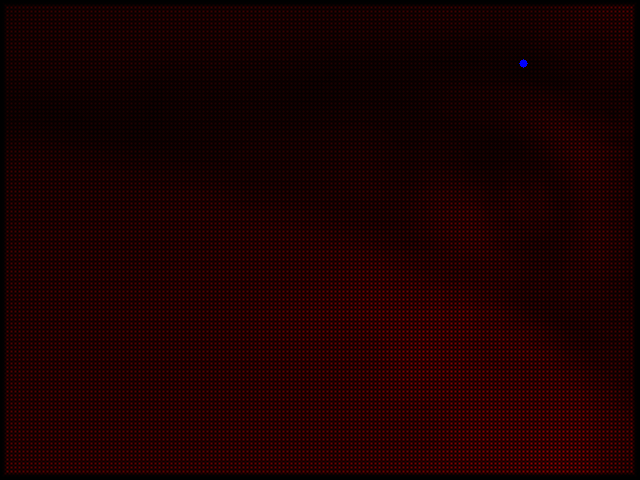
\includegraphics[width=0.9\linewidth]{plots/results/responsehaarworst.png}
        \caption{feature vector result with best response}
    \end{subfigure}%
 
    \caption{Limits to the Haar-like feature approach}
    \label{fig:limit_haar}
\end{figure}
The problem with the LPW data set is, that it is so versatile and the conditions change during the recording. This makes it hard to find an approach that can adapt to all the conditions and still perform well in a given time interval. The implementation can still be improved and sped up, in the Haar-like feature the following libraries were used to speed up the algorithm: 

\begin{python}
from concurrent.futures import ThreadPoolExecutor
from numba import njit
    \end{python}
ThreadPool Executor makes it possible to use multithreading and njit compiles the sliding window over the integral image of the Haar-like feature to machine code for more efficient calculation.

\subsection{Ellipse parameter estimation}
In the second part of an pupil detection algorithm it is necessary to make use of the informations from the first part and build on this foundation and find the five ellipse parameter: center: $(x,y)$, axis: (major, minor) and angle. The LPW has labels for the center only of the pupil and therefore only the center can be used to evaluate the performance of the algorithms. A second evaluation has to be done manually by inspecting the fit of the ellipse to the pupil. This is hard to evaluate with numerical methods and the result needs therefore to be taken with a grain of salt. In this section 4 different algorithms will be discussed and evaluated: The OpenCV ellipse fit based on contours (binary thresholding), ACWE with OpenCV Ellipse fit, ACWE combined with RANSAC, and Canny edge detection with OpenCV Ellipse fit. 

